
从并发性的角度来看,\textbf{堆栈}是最简单的数据结构之一。堆栈上的所有操作都处理顶部元素,因此(至少在概念上)需要保护一个位置以防止竞争。

C++标准库为我们提供了\texttt{std::stack}容器,可以将该容器作为一个起点。所有C++容器,都提供了弱线程安全:多个线程可以安全地访问只读容器。换句话说,只要没有线程调用非\texttt{const}函数,任何数量的线程都可以同时调用任何\texttt{const}方法。虽然这听起来很简单,几乎过于简单,但这里有一个问题:在最后一次修改和只读的部分之间,必须存在某种同步。换句话说,所有线程在内存栅栏之前执行,写访问并没有真正完成:写线程至少必须释放内存,而读线程必须获取内存。任何强栅栏都可以工作,锁也可以,但每个线程都必须迈出这一步。

\subsubsubsection{7.3.1\hspace{0.2cm}线程安全的接口设计}

现在,如果多个线程在修改堆栈,则需要更强的保证,那该怎么办?提供互斥锁的最直接的方法,用互斥锁保护类的每个成员函数。这可以在应用程序级别完成,但是这样的实现并不是强线程安全,很容易出错。因为锁与容器没有关联,也很难进行调试和分析。

更好的选择是用自己的类包装堆栈类:

\hspace*{\fill} \\ %插入空行
\noindent
\textbf{02\_stack.C}
\begin{lstlisting}[style=styleCXX]
template <typename T> class mt_stack {
	std::stack<T> s_;
	std::mutex l_;
	public:
	mt_stack() = default;
	void push(const T& v) {
		std::lock_guard g(l_);
		s_.push(v);
	}
	…
};
\end{lstlisting}

注意,可以使用继承而不是封装。这样做会使编写\texttt{mt\_stack}的构造函数更容易,只需要一个\texttt{using}语句。但是,使用公共继承会公开基类\texttt{std::stack}的每个成员函数,若忘记包装其中一个,代码将编译,将直接调用未保护的成员函数。私有(或受保护的)继承避免了这个问题,但会带来其他危险。有些构造函数需要重新实现,例如:移动构造函数需要锁定正在被移动的堆栈,因此需要自定义实现。在没有包装器的情况下,公开其他几个构造函数十分危险,因为它们会读取或修改参数。总的来说,必须重写想要提供的每个构造函数,这样比较安全。这与C++的建议是一致的:组合优于继承(\textit{prefer composition over inheritance})。

我们的线程安全或多线程堆栈(就是\textit{mt}的意思)现在有了\textit{push}功能,并准备接收数据。我们只需要逆操作\textit{pop}。我们当然可以按照前面的例子包装\texttt{pop()},但这还远远不够:STL堆栈使用三个独立的成员函数从堆栈中删除元素。\texttt{pop()}删除了顶部元素,但没有任何返回.所以想知道堆栈顶部是什么,必须首先使用\texttt{top()}。如果堆栈为空,那么使用这两种方法中的任何一个都会导致未定义行为,所以必须首先使用\texttt{empty()}检查结果。我们可以包装这三个方法,这里先不展示。下面的代码中,假设堆栈的所有成员函数都由一个锁保护:

\begin{lstlisting}[style=styleCXX]
mt_stack<int> s;
… push some data on the stack …
int x = 0;
if (!s.empty()) {
	x = s.top();
	s.pop();
}
\end{lstlisting}

每个成员函数都是线程安全的,但在多线程上下文中完全无用:堆栈可能在某一刻(碰巧使用\texttt{s.empty()}的那一刻)非空,但在下一刻(调用\texttt{s.top()}之前)就变成空的了,因为在此期间另一个线程可以删除顶部的元素。

这可能是整本书最重要的内容了。为了提供可用的线程安全的功能,在选择接口时必须考虑线程安全,但不能在现有的设计上添加线程安全特性。而在进行设计时,必须考虑到线程安全。因为可以选择在设计中提供某些保证和不变量,这些在并发程序中不可维护,例如:\texttt{std::stack}保证调用\texttt{empty()}是安全的,并返回false,这样就可以安全地调用\texttt{top()},只要在这两个调用之间不做任何其他的堆栈操作就好。在多线程程序中,没有特别好的方法来履行这种承诺。

幸运的是,由于我们正在编写自己的包装器类,所以不需要逐个使用包装类的接口。那么,我们应该怎么做呢?显然,整个\texttt{pop}操作是一个成员函数,应该从堆栈中删除顶部元素,并将其返回给调用者。问题是当堆栈为空时该做什么?有多种选择。可以返回一对值和一个布尔标志,该标志指示堆栈是否为空(在这种情况下,该值必须有默认构造)。也可以单独返回布尔值,并通过引用传递该值(如果堆栈为空,则该值保持不变)。在C++ 17中,解决方案是返回\texttt{std::optional},如以下代码所示。它非常适合持有可能并不存在的值:

\hspace*{\fill} \\ %插入空行
\noindent
\textbf{02\_stack.C}
\begin{lstlisting}[style=styleCXX]
template <typename T> class mt_stack {
	std::stack<T> s_;
	std::mutex l_;
	public:
	std::optional<T> pop() {
		std::lock_guard g(l_);
		if (s_.empty()) {
			return std::optional<T>(std::nullopt);
		} else {
			std::optional<T> res(std::move(s_.top()));
			s_.pop();
			return res;
		}
	}
};
\end{lstlisting}

如你所见,将元素从堆栈中弹出的整个操作现在都受到锁的保护。这个接口是事务性的:每个成员函数将对象从一个已知状态转到另一个已知状态。

如果对象必须转换到一些中间状态,比如使用\texttt{empty()}之后,并在使用\texttt{pop()}之前的状态,这些状态必须对使用者不可见。相反,向使用者呈现的是单个原子事务:要么返回顶部的元素,要么通知调用者不能进行该操作,这确保了程序的正确性。现在,我们来看看性能。

\subsubsubsection{7.3.2\hspace{0.2cm}使用互斥的性能}

堆栈的性能如何?假设每个操作从开始到结束都是锁定的,那就不要对堆栈成员函数的性能有什么期待。最好的情况下线程都将串行地执行堆栈操作,但在实际中,我们应该预计到锁会带来一些开销。如果要比较多线程堆栈和普通\texttt{std::stack}的性能,我们可以在基准测试中进行对比。

为了简化基准测试,可以选择在\texttt{std::stack}上实现单线程的非阻塞包装器,该包装器提供与\texttt{mt\_stack}相同的接口。注意,不能仅通过推入堆栈来进行基准测试,这样基准测试可能会将内存耗尽。类似地,无法可靠地对弹出操作进行基准测试,除非想测量从空堆栈弹出的耗时。如果基准测试运行的时间足够长,就必须将推和弹结合起来。最简单的基准可以是这样的:

\hspace*{\fill} \\ %插入空行
\noindent
\textbf{02\_stack.C}
\begin{lstlisting}[style=styleCXX]
mt_stack<int> s;
void BM_stack(benchmark::State& state) {
	const size_t N = state.range(0);
	for (auto _ : state) {
		for (size_t i = 0; i < N; ++i) s.push(i);
		for (size_t i = 0; i < N; ++i)
		benchmark::DoNotOptimize(s.pop());
	}
	state.SetItemsProcessed(state.iterations()*N);
}
\end{lstlisting}

当运行多线程时,有可能在堆栈为空时进行\texttt{pop()}操作。对于处于设计阶段的堆栈来说,这可能是现实的。此外,由于基准测试仅向我们提供了真实应用程序中数据结构性能的近似值,其中的差异可以忽略。为了获得更精确的测量值,必须模拟应用程序,并执行真实的\texttt{push}和\texttt{pop}操作序列。结果应该是这样的:

%\hspace*{\fill} \\ %插入空行
\begin{center}
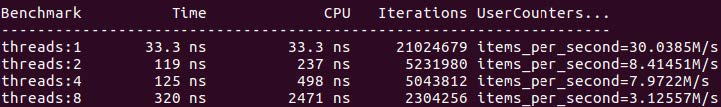
\includegraphics[width=0.9\textwidth]{content/2/chapter7/images/3.jpg}\\
图7.3 - 锁栈——使用互斥锁——的性能
\end{center}

注意这里的“item”是“一个push,后面跟着一个pop”操作,所以“items per second”的值显示了每秒钟可以通过堆栈发送多少数据。为了进行比较,没有锁的堆栈在单个线程上的执行速度要比使用互斥锁快10倍多:

%\hspace*{\fill} \\ %插入空行
\begin{center}
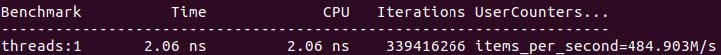
\includegraphics[width=0.9\textwidth]{content/2/chapter7/images/4.jpg}\\
图7.4 - \texttt{std::stack}的性能(与图7.3相比)
\end{center}

如我们所见,使用互斥对象实现的堆栈性能相当差。但是,不要急于找到或设计一些聪明的线程安全堆栈,至少现在还不需要。这时,应该问的第一个问题是,这是咋回事?应用程序如何处理堆栈上的数据?例如,如果每个数据元素都需要耗时几秒钟模拟一个参数,那么堆栈的速度就不重要了。另一方面,如果堆栈位于某些实时事务处理系统的核心,那么它的速度可能是整个系统性能的关键。

顺便说一下,结果可能与其他数据结构类似,如列表、双端队列、队列和树。其中,单个操作要比对互斥锁的操作快得多。但是,在尝试改进性能之前,我们必须准确地了解应用程序需要什么样的性能。

\subsubsubsection{7.3.3\hspace{0.2cm}不同的性能需求}

本章的其余部分中,我们会假设数据结构的性能在应用程序中很重要。现在,可以来聊聊最快的堆栈实现了吗?还没到那个时候。我们还需要考虑使用的模型。换句话说,我们该如何处理堆栈,以及什么才是真正需要加速的东西。

正如刚才看到的,互斥锁堆栈性能较差的关键原因是,速度基本上受到互斥锁的限制,对堆栈操作进行基准测试几乎与对互斥锁的锁定和解锁进行基准测试结果相同。提高性能的一种方法是改进互斥锁的实现,或者使用另一种同步方案。另一种方法是少使用互斥锁,这要求我们重新设计客户端代码。

例如,使用者通常有多个必须压入堆栈的项。类似地,使用者可以一次从堆栈中弹出几个元素并进行处理。这种情况下,可以使用数组或容器来实现批量推送或批量弹出,以便一次从堆栈中复制多个元素。由于锁定的开销很大,我们可以用锁定/解锁操作在堆栈上一次性推入1024个元素,这样就比用锁时一个一个推入元素来的快。事实上,基准测试也反映了这一点:

%\hspace*{\fill} \\ %插入空行
\begin{center}
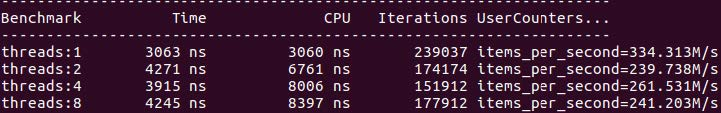
\includegraphics[width=0.9\textwidth]{content/2/chapter7/images/5.jpg}\\
图7.5 - 批处理堆栈操作的性能(每个锁1,024个元素)
\end{center}

我们应该非常清楚这种方式可以做哪些事,不能做哪些事:若临界区内的操作比锁操作本身快得多,就该减少锁的开销,但不能锁定操作的规模。此外,通过延长停留在临界区的时间,迫使线程在锁上等待更长时间。如果所有线程都尝试访问堆栈(这就是基准测试变得更快的原因),那么没问题。但是,若在我们的应用程序中,线程主要是执行其他计算,只是偶尔访问堆栈,那么较长的等待可能会降低整体性能。为了明确地回答批量\texttt{push}和批量\texttt{pop}是否对性能有益,我们必须在更真实的环境中对它们进行分析。

其他一些场景中,寻找更有限的、特定于应用程序的解决方案,可以获得远高于通用解决方案的改进实现所能获得的性能收益。例如,这种场景在某些应用程序中很常见:单个线程将大量数据提前\texttt{push}到堆栈上,然后多个线程将数据从堆栈中删除并处理,可能还会将更多数据\texttt{push}到堆栈上。这种情况下,可以实现解锁的\texttt{push},只在前置\texttt{push}的单线程中使用。虽然使用者的责任是永远不要在多线程中使用这个方法,但解锁的堆栈比锁定的堆栈快得多,因此这里的复杂性可能是值得的。

更复杂的数据结构提供了各种各样的使用模型,但即使是堆栈也可以使用,而不仅仅是简单的\texttt{push}和\texttt{pop}。我们也可以查看顶部的元素而不删除。\texttt{std::stack}提供了\texttt{top()}成员函数,但它不是事务性的,所以我们必须创建自己的函数。它非常类似于事务性的\texttt{pop()}函数,只是不移除顶部的元素:

\hspace*{\fill} \\ %插入空行
\noindent
\textbf{02\_stack.C}
\begin{lstlisting}[style=styleCXX]
template <typename T> class mt_stack {
	std::stack<T> s_;
	mutable std::mutex l_;
	public:
	std::optional<T> top() const {
		std::lock_guard g(l_);
		if (s_.empty()) {
			return std::optional<T>(std::nullopt);
		} else {
			std::optional<T> res(s_.top());
			return res;
		}
	}
};
\end{lstlisting}

注意,为了允许只进行查找\texttt{top()}声明为\texttt{const},这里必须将互斥量声明为\texttt{mutable}。这样做时要小心:多线程程序的约定是遵循STL,只要不调用非\texttt{const}成员函数,所有\texttt{const}成员函数都可以安全地在多个线程上使用。这意味着\texttt{const}函数不会修改对象是只读的,而可变数据成员违背了这个假设。至少,它们不应该表示对象的逻辑状态。然后,在修改时应该小心避免竞争条件。互斥锁满足这两个要求。

现在可以考虑不同的使用模式。在某些应用程序中,数据\texttt{push}入堆栈,再从中\texttt{pop}出。其他情况下,堆顶元素可能需要在每次\texttt{push}和\texttt{pop}之间检查多次。我们先关注后一种情况,而后再次检查\texttt{top()}的代码。这里有一个明显的低效存在:由于锁的存在,在任何时刻只有一个线程可以读取栈顶元素。但是读取顶部元素是一个非修改(只读)操作。如果所有线程都这样做,并且没有线程同时尝试修改堆栈,那么根本就不需要锁。但现在,它的性能与\texttt{pop()}一样。

不能在\texttt{top()}中省略锁的原因是,不能确定另一个线程在同一时间没有使用\texttt{push()}或\texttt{pop()}。但即使这样,也不需要对\texttt{top()}的两次锁定,它们可以同时进行。只有修改堆栈的操作需要锁定。有一种类型的锁提供这样的功能,通常被称为\textbf{读写锁}。任何数量的线程都可以获得读锁,并且这些线程之间不会互相影响。但是,写锁只能由一个线程获得,而且只有在没有其他线程持有读锁的情况下才能获取。在C++中,术语不同(但功能完全相同):读线程使用共享锁(同一个互斥对象上的共享锁可以同时存在),但写线程需要唯一锁(给定的互斥对象上只能存在一个这样的锁)。如果另一个线程已经持有唯一的锁,那么获取共享锁的尝试将会阻塞。同样,若另一个线程持有同一个互斥对象上的锁,那么获取唯一锁的尝试将会阻塞。有了共享互斥锁,就可以用我们需要的那种锁来实现堆栈。\texttt{top()}使用了共享锁,因此任意数量的线程都可以同时执行,但\texttt{push()}和\texttt{pop()}则需要唯一锁:

\begin{lstlisting}[style=styleCXX]
template <typename T> class rw_stack {
	std::stack<T> s_;
	mutable std::shared_mutex l_;
	public:
	void push(const T& v) {
		std::unique_lock g(l_);
		s_.push(v);
	}
	std::optional<T> pop() {
		std::unique_lock g(l_);
		if (s_.empty()) {
			return std::optional<T>(std::nullopt);
		} else {
			std::optional<T> res(std::move(s_.top()));
			s_.pop();
			return res;
		}
	}
	std::optional<T> top() const {
		std::shared_lock g(l_);
		if (s_.empty()) {
			return std::optional<T>(std::nullopt);
		} else {
			std::optional<T> res(s_.top());
			return res;
		}
	}
};
\end{lstlisting}

不幸的是,我们的基准测试显示,使用\texttt{top()}的性能即使在读写锁下也不会改变:

%\hspace*{\fill} \\ %插入空行
\begin{center}
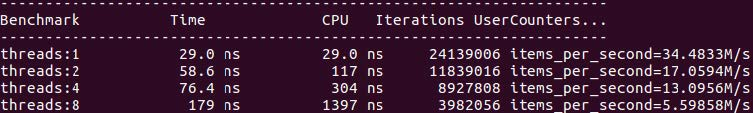
\includegraphics[width=0.9\textwidth]{content/2/chapter7/images/6.jpg}\\
图7.6 - 使用\texttt{std::shared\_mutex}的栈性能——只读操作
\end{center}

更糟糕的是,与普通互斥锁相比,唯一锁的性能下降得更厉害::

%\hspace*{\fill} \\ %插入空行
\begin{center}
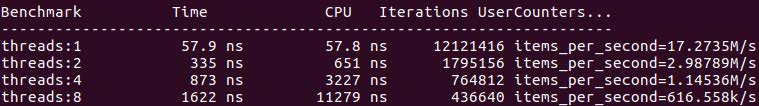
\includegraphics[width=0.9\textwidth]{content/2/chapter7/images/7.jpg}\\
图7.7 - 使用\texttt{std::shared\_mutex}栈的性能——写入操作
\end{center}

将图7.6和7.7与图7.4中早期测量值进行比较,可以看到读写锁并没有带来任何改进。这个结论并不普遍,因为不同互斥体的性能取决于实现和硬件。然而,更复杂的锁,比如共享互斥锁,会比简单锁有更多的开销。它们的目标程序是不同的:如果临界区内的操作花费的时间长得多(比如,毫秒而不是微秒),并且大多数线程执行只读代码,那么不锁定只读线程将会有很大的价值,而且几微秒的操作开销将会少得多。

观察更长的临界段是非常重要的:如果堆栈元素较大,并且复制的代价非常昂贵,那么与复制大对象的代价相比,锁的性能就不重要了。但是,假设我们的总体目标是使程序快速,而不是展示可扩展的堆栈实现,我们将通过消除昂贵的复制,并使用指针堆栈来优化整个应用程序。

尽管读写锁遇到了挫折,但我们正确的走在实现更高效应用的路上。在设计之前,我们必须更详细地了解每个堆栈操作的作用,以及在每个步骤中必须避免可能出现的数据竞争。

\subsubsubsection{7.3.4\hspace{0.2cm}堆栈性能详情}

As we try to improve the performance of the thread-safe stack (or any other data structure) beyond that of the simple lock-guarded implementation, we have to first understand in detail the steps involved in each operation and how they may interact with other operations executed on different threads. The main value of this section is not the faster stack but this analysis: it turns out that these low-level steps are common to many data structures. Let's start with the push operation. Most stack implementations are built on top of some array-like container, so let's view the top of the stack as a contiguous block of memory:

\hspace*{\fill} \\ %插入空行
\begin{center}
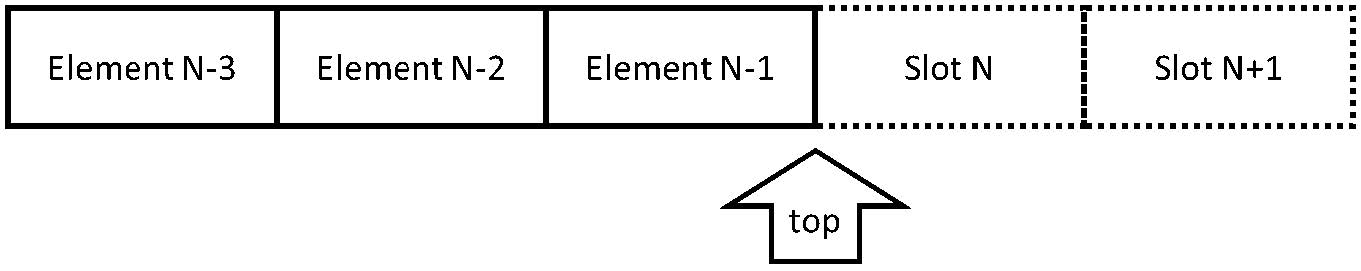
\includegraphics[width=0.9\textwidth]{content/2/chapter7/images/8.jpg}\\
Figure 7.8 – Top of the stack for push operation
\end{center}

There are N elements on the stack, so the element count is also the index of the first free slot where the next element would go. The push operation must increment the top index (which is also the element count) from N to N+1 to reserve its slot and then construct the new element in the slot N. Note that this top index is the only part of the data structure where the threads doing push can interact with each other: as long as the index increment operation is thread-safe, only one thread can see each value of the index. The first thread to execute the push advances the top index to N+1 and reserves the Nth slot, the next thread increments the index to N+2 and reserves the N+1st slot, and so on. The key point here is that there is no race for the slots themselves: only one thread can get a particular slot, so it can construct the object there without any danger of another thread interfering with it.

This suggests a very simple synchronization scheme for the push operations: all we need is a single atomic value for the top index:

\begin{lstlisting}[style=styleCXX]
std::atomic<size_t> top_;
\end{lstlisting}

A push operation atomically increments this index and then constructs the new element in the array slot indexed by the old value of the index:

\begin{lstlisting}[style=styleCXX]
const size_t top = top_.fetch_add(1);
new (&data[top]) Element(… constructor arguments … );
\end{lstlisting}

Again, there is no need to protect the construction step from other threads. The atomic index is all we need to make the push operations thread-safe. By the way, this is true if we use an array as the stack memory. If we use a container such as std::deque, we cannot simply construct a new element over its memory: we have to call push\_back to update the size of the container, and that call is not thread-safe even if the deque does not need to allocate more memory. For this reason, data structure implementations that go beyond basic locks usually also have to manage their own memory. Speaking of memory, we have assumed so far that the array has space to add more elements, and we do not run out of memory. Let's stick with this assumption for now.

What we have so far is a very efficient way to implement a thread-safe push operation in a particular case: multiple threads may be pushing data onto the stack, but nobody is reading it until all push operations are done.

The same idea works if we have a stack with elements already pushed onto it, and we need to pop them (and no more new elements are added). Figure 7.8 works for this scenario as well: a thread atomically decrements the top count and then returns the top element to the caller:

\begin{lstlisting}[style=styleCXX]
const size_t top = top_.fetch_sub(1);
return std::move(data[top]);
\end{lstlisting}

The atomic decrement guarantees that only one thread can access each array slot as the top element. Of course, this works only as long as the stack is not empty. We could change the top element index from an unsigned to a signed integer; then, we would know that the stack is empty when the index becomes negative.

This is, again, a very efficient way to implement thread-safe pop operation under very special conditions: the stack is already populated, and no new elements are added. In this case, we also know how many elements are on the stack, so it is fairly easy to avoid an attempt to pop the empty stack.

In some specific applications, this may be of some value: if the stack is first populated by multiple threads without any pops and there is a clearly defined point in the program where it switches from adding data to removing it, then we have a great solution for each half of the problem. But let's continue to a more general case.

Our very efficient push operation is, unfortunately, of no help when it comes to reading from the stack. Let's consider again how we would implement the operation that pops the top element. We have the top index, but all it tells us is how many elements are currently being constructed; it says nothing about the location of the last element whose construction is completed (element N-3 in Figure 7.9):

\hspace*{\fill} \\ %插入空行
\begin{center}
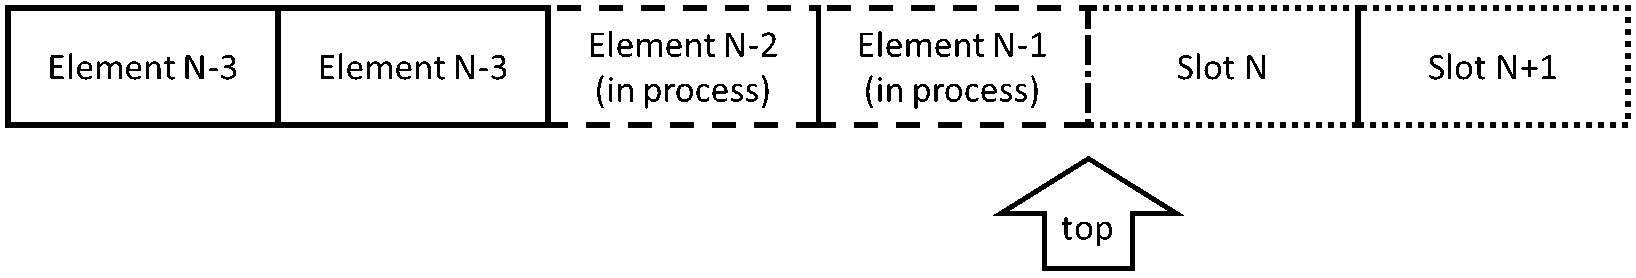
\includegraphics[width=0.9\textwidth]{content/2/chapter7/images/9.jpg}\\
Figure 7.9 – Top of the stack for push and pop operations
\end{center}

Of course, the thread that does the push and, therefore, the construction, knows when it's done. Perhaps what we need is another count that shows how many elements are fully constructed. Alas, if only it was that simple. In Figure 7.9, let's assume that thread A is constructing the element N-2 and that thread B is constructing the element N-1. Obviously, thread A was the first to increment the top index. But it doesn't mean it will also be the first to complete the push. Thread B may finish the construction first. Now, the last constructed element on the stack has the index N-1, so we could advance the constructed count to N-1 (note that we jumped over element N-2, which is still in the middle of the construction). Now we want to pop the top element; no problem, the element N-1 is ready, and we can return it to the caller and remove it from the stack; the constructed count is now decremented to N-2. Which element should we pop next? The element N-2 is still not ready, but nothing in our stack warns us about it. We have only one count for completed elements, and its value is N-1. Now we have a data race between the thread that constructs a new element on the stack and the thread that tried to pop it.

Even without this race, there is another problem: we just popped the element N-1, which was the right thing to do at the time. But while that was happening, a push was requested on thread C. Which slot should be used? If we use slot N-1, we risk overwriting the same element that is currently being accessed by thread A. If we use slot N, then, once all the operations are completed, we have a hole in the array: the top element is N, but the next one is not N-1: it was already popped, and we have to jump over it. Nothing in this data structure tells us that we must do so.

We could keep track of which elements are real and which ones are holes, but this is becoming more and more complex (and doing it in a thread-safe manner will require additional synchronization that will reduce performance). Also, leaving many array slots unused wastes memory. We could attempt to reuse the holes for new elements pushed on the stack, but at this point, the elements are no longer stored consecutively, the atomic top count no longer works, and the whole structure begins to resemble a list. By the way, if you think that a list would be a great way to implement a thread-safe stack, wait until you see what it takes to implement a thread-safe list later in this chapter.

At this point in our design, we must pause the deep dive into the implementation details and again review the more general approach to the problem. There are two steps that we must do: generalize the conclusions from our deeper understanding of the details of the stack implementations and do some performance estimates to get a general idea about what solutions are likely to yield performance improvements. We will start with the latter.

\subsubsubsection{7.3.5\hspace{0.2cm}同步方案的性能评估}

Our first attempt at a very simple stack implementation without a lock yielded some interesting solutions for special cases but no general solution. Before we spend much more time building a complex design, we should try to estimate how likely is it that it is going to be more efficient than the simple lock-based one.

Of course, this may seem like circular reasoning: in order to estimate the performance, we must first have something to estimate. But we don't want to do the complex design without at least some assurances that the effort will pay off, the assurances that require a performance estimate.

Fortunately, we can fall back on the general observations we learned earlier: the performance of concurrent data structures depends largely on how many shared variables are accessed concurrently. Let's assume that we can come up with a clever way to implement the stack with a single atomic counter. It is reasonable to assume that every push and pop will have to do at least one atomic increment or decrement of this counter (unless we are doing batch operations, but we already know that they are faster). We can get a reasonable performance estimate if we make a benchmark that combines push and pop on the single-threaded stack with an atomic operation on a shared atomic counter. There is no synchronization going on, so we have to use a separate stack for every thread to avoid race conditions:

\begin{lstlisting}[style=styleCXX]
std::atomic<size_t> n;
void BM_stack0_inc(benchmark::State& state) {
	st_stack<int> s0;
	const size_t N = state.range(0);
	for (auto _ : state) {
		for (size_t i = 0; i < N; ++i) {
			n.fetch_add(1, std::memory_order_release);
			s0.push(i);
		}
		for (size_t i = 0; i < N; ++i) {
			n.fetch_sub(1, std::memory_order_acquire);
			benchmark::DoNotOptimize(s0.pop());
		}
	}
	state.SetItemsProcessed(state.iterations()*N);
}
\end{lstlisting}

Here, st\_stack is a stack wrapper that presents the same interface as our lock-based mt\_stack but without any locks. The real implementation is going to be somewhat slower because the stack top is also shared between threads, but this will give us an estimate from above: it is highly unlikely that any implementation that is actually threadsafe will outperform this artificial benchmark. What do we compare the results to? The benchmark of the lock-based stack in Figure 7.3 shows the performance of the lock-based stack to be between 30M push/pop operations per second on one thread and 3.1M on 8 threads. We also know the baseline performance of the stack without any locks to be about 485M operations per second (Figure 7.4). On the same machine, our performance estimate with a single atomic counter yields these results:

\hspace*{\fill} \\ %插入空行
\begin{center}
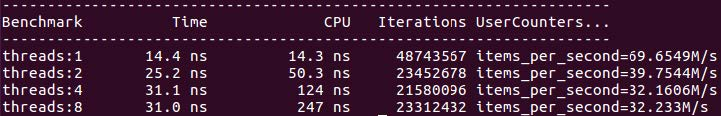
\includegraphics[width=0.9\textwidth]{content/2/chapter7/images/10.jpg}\\
Figure 7.10 – Performance estimate of a hypothetical stack with a single atomic counter
\end{center}

The result seems like a mixed bag: even under optimal conditions, our stack is not going to scale. Again, this is primarily because we are testing a stack of small elements; if the elements were large and expensive to copy, we would see scaling because multiple threads can copy data at the same time. But the earlier observation stands: if copying data becomes so expensive that we need many threads to do it, we are better off using a stack of pointers and not copying any data at all.

On the other hand, the atomic counter is much faster than the mutex-based stack. Of course, this is an estimate from above, but it suggests that a lock-free stack has some possibilities. However, so does the lock-based stack: there are more efficient locks than std::mutex when we need to lock very short critical sections. We had already seen one such lock in Chapter 6, Concurrency and Performance, when we implemented a spinlock. If we use this spinlock in our lock-based stack, then, instead of Figure 7.2, we get these results:

\hspace*{\fill} \\ %插入空行
\begin{center}
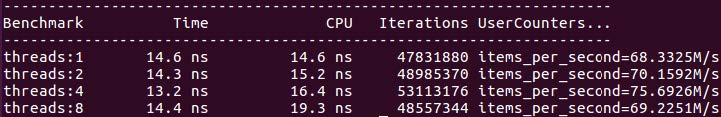
\includegraphics[width=0.9\textwidth]{content/2/chapter7/images/11.jpg}\\
Figure 7.11 – Performance of the spinlock-based stack
\end{center}

Comparing this result with Figure 7.10 paints a very depressing picture: we are not going to come up with a lock-free design that can outperform a simple spinlock. The reason that the spinlock can outperform an atomic increment in some cases has to do with the relative performance of different atomic instructions on this particular hardware; we should not read too much into it.

We could try to do the same estimate with an atomic exchange or compare-and-swap instead of the atomic increment. As you learn more about designing thread-safe data structures, you will get a sense of which synchronization protocol is likely to be useful and what operations should go into the estimate. Also, if you work with particular hardware, you should run simple benchmarks to determine which operations are more efficient on it. All results so far were obtained on X86-based hardware. If we run the same estimates on a large ARM-based server designed specifically for HPC applications, we get a very different outcome. The benchmark of a lock-based stack yields these results:

\hspace*{\fill} \\ %插入空行
\begin{center}
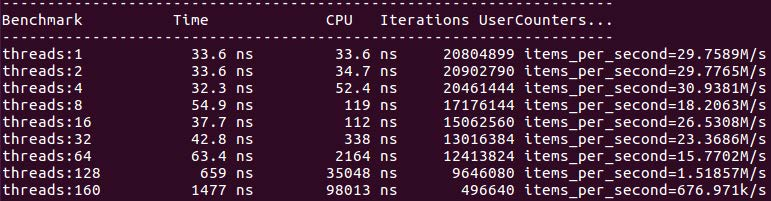
\includegraphics[width=0.9\textwidth]{content/2/chapter7/images/12.jpg}\\
Figure 7.12 – Performance of the lock-based stack on an ARM HPC system
\end{center}

The ARM systems typically have a much larger number of cores than X86 systems, while the performance of a single core is lower. This particular system has 160 cores on two physical processors, and the performance of the lock drops significantly when the program runs on both CPUs. The estimate for the upper limit of the lock-free stack performance should be done with a compare-and-swap instruction instead of the atomic increment (the latter is particularly inefficient on these processors).

\hspace*{\fill} \\ %插入空行
\begin{center}
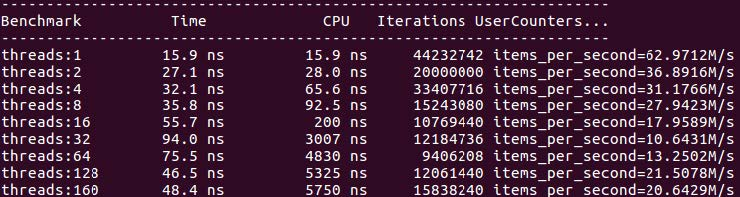
\includegraphics[width=0.9\textwidth]{content/2/chapter7/images/13.jpg}\\
Figure 7.13 – Performance estimate for a hypothetical stack with a single CAS operation (ARM processors)
\end{center}

Based on the estimates in Figure 7.13, there is a chance that, for a large number of threads, we can come up with something better than a simple lock-based stack. We are going to continue with our efforts to develop a lock-free stack. There are two reasons for it: first of all, this effort is ultimately going to pay off on some hardware. Second, the basic elements of this design will be seen later in many other data structures, and the stack offers us a simple test case for learning about them.

\subsubsubsection{7.3.6\hspace{0.2cm}无锁的堆栈}

Now that we have decided to try and outperform a simple lock-based implementation, we need to consider the lessons we have learned from our exploration of the push and pop operations by themselves. Each operation is very simple by itself, but the interaction of the two is what creates complexity. This is a very common situation: it is much harder to correctly synchronize producer and consumer operations running on multiple threads than it is to handle only producers or only consumers. Remember this when designing your own data structures: if your application allows for any kind of limitation on the operations you need to support, such as producers and consumers are separate in time, or there is a single producer (or consumer) thread, you can almost certainly design a faster data structure for these limited operations.

Assuming that we need a fully generic stack, the essence of the problem of the producerconsumer interaction can be understood on a very simple example. Again, we assume that the stack is implemented on top of an array or an array-like container, and the elements are stored consecutively. Let's say that we have N elements currently on the stack. The producer thread P is executing the push operation, and the consumer thread C is executing the pop operation at the same time. What should be the outcome? While it is tempting to try to come up with a wait-free design (like we did for only consumers or only producers), any design that allows both threads to proceed without waiting is going to break our fundamental assumption about how the elements are stored: the thread C has to either wait for the thread P to complete the push or return the current top element, N. Similarly, the thread P has to either wait for the thread C to complete or construct a new element in the slot N+1. If neither thread waits, the result is a hole in the array: the last element has the index N+1, but there is nothing stored in the slot N, so we must somehow skip it when we pop data from the stack.

It looks like we have to give up the idea of the wait-free stack implementation and make one of the threads wait for the other one to complete its operation. We also have to deal with the possibility of the empty stack when the top index is zero and a consumer thread attempts to further decrement it. A similar problem occurs at the upper bound of the array when the top index points to the last element and a producer thread needs another slot.

Both of these problems require a bounded atomic increment operation: perform the increment (or decrement) unless the value equals the specified bound. There is no readymade atomic operation for this in C++ (or on any mainstream hardware available today), but we can implement it using compare-and-swap (CAS) as follows:

\begin{lstlisting}[style=styleCXX]
std::atomic<int> n_ = 0;
int bounded_fetch_add(int dn, int maxn) {
	int n = n_.load(std::memory_order_relaxed);
	do {
		if (n + dn >= maxn || n + dn < 0) return -1;
	} while (!n_.compare_exchange_weak(n, n + dn,
			std::memory_order_release,
			std::memory_order_relaxed));
	return n;
}
\end{lstlisting}

This is a typical example of how CAS operation is used to implement a complex lock-free atomic operation:

\begin{enumerate}
\item Read the current value of the variable.
\item Check the necessary conditions. In our case, we verify that the increment would not give us the value outside of the specified bounds [0, maxn). If the bounded increment fails, we signal it to the caller by returning -1 (this is an arbitrary choice; usually, there is a specific action to be performed for the out-of-bounds case).
\item Atomically replace the value with the desired result if the current value is still equal to what we read earlier.
\item If step 3 failed, the current value has been updated, check it again, and repeat steps 3 and 4 until we succeed.
\end{enumerate}

While this may seem to be a kind of lock, there is a fundamental difference: the only way the CAS comparison can fail on one thread is if it succeeded (and the atomic variable was incremented) on another thread, so any time there is a contention for the shared resource, at least one thread is guaranteed to make forward progress.

There is one more important observation that often makes all the difference between a scalable implementation and a very inefficient one. The CAS loop, as written, is very hostile to the scheduling algorithms of most modern operating systems: the thread that loops unsuccessfully also consumes more CPU time and will be given higher priority. This is the exact opposite of what we want: we want the thread that is currently doing the useful work to run faster. The solution is for a thread to yield the scheduler after a few unsuccessful CAS attempts. This is accomplished by a system call that is OS-dependent, but C++ has a system-independent API via the call to std::this\_thread::yield(). On Linux, usually one can get better performance by calling the nanosleep() function to sleep for the minimum possible time (1 nanosecond) every few iterations of the loop:

\begin{lstlisting}[style=styleCXX]
int i = 0;
while ( … ) {
	if (++i == 8) {
		static constexpr timespec ns = { 0, 1 };
		i = 0;
		nanosleep(&ns, NULL);
	}
}
\end{lstlisting}

The same approach can be used to implement much more complex atomic transactions, such as stack push and pop operations. But first, we have to figure out what atomic variables are needed. For the producer threads, we need the index of the first free slot in the array. For the consumer threads, we need the index of the last fully constructed element. This is all the information we need about the current state of the stack, assuming we do not allow "holes" in the array:

\hspace*{\fill} \\ %插入空行
\begin{center}
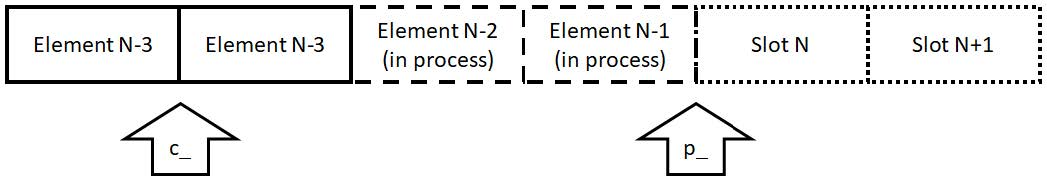
\includegraphics[width=0.9\textwidth]{content/2/chapter7/images/14.jpg}\\ Figure 7.14 – Lock-free stack: c\_ is the index of the last fully constructed element, and p\_ is the index of the first free slot in the array
\end{center}

First of all, neither push nor pop can proceed if the two indices are currently not equal: different counts imply that either a new element is being constructed or the current top element is being copied out. Any stack modification in this state may lead to the creation of holes in the array.

If the two indices are equal, then we can proceed. To do the push, we need to atomically increment the producer index p\_ (bounded by the current capacity of the array). Then we can construct the new element in the slot we just reserved (indexed by the old value of p\_). Then we increment the consumer index c\_ to indicate that the new element is available to the consumer threads. Note that another producer thread could grab the next slot even before the construction is completed, but we would have to wait until all new elements are constructed before we allow any consumer thread to pop an element. Such an implementation is possible, but it is more complex, and it tends to favor the currently executed operation: if a push is currently in progress, a pop has to wait, but another push can proceed without delay. The result is likely to be a swarm of push operations executing while all consumer threads are waiting (the effect is similar if a pop operation is in progress; it favors another pop).

The pop is implemented similarly, only we first decrement the consumer index c\_ to reserve the top slot, and then decrement p\_ after the object is copied or moved from the stack.

There is just one more trick we have to learn, and that is how to manipulate both counts atomically. For example, we said earlier that a thread has to wait for the two indices to become equal. How can this be accomplished? If we read one index atomically and then the other index, also atomically, there is a chance that the first index has changed since we read it. We have to read both indices in a single atomic operation. The same is true for other operations on the indices. C++ allows us to declare an atomic struct of two integers; however, we must be careful: very few hardware platforms have a double CAS instruction that operates on two long integers atomically, and even then, it is usually very slow. The better solution is to pack both values into a single 64-bit word (on a 64-bit processor). The hardware atomic instructions such as load or compare-and-swap do not really care how you are going to interpret the data they read or write: they just copy and compare 64-bit words. You can later treat these bits as a long or a double or a pair of ints (the atomic increment is, of course, different, which is why you cannot use it on a double value).

Now, all that is left is to convert the preceding algorithm into code:

\hspace*{\fill} \\ %插入空行
\noindent
\textbf{02b\_stack\_cas.C}
\begin{lstlisting}[style=styleCXX]
template <typename T> class mt_stack {
	std::deque<T> s_;
	int cap_ = 0;
	struct counts_t {
		int p_ = 0; // Producer index
		int c_ = 0; // Consumer index
		bool equal(std::atomic<counts_t>& n) {
			if (p_ == c_) return true;
			*this = n.load(std::memory_order_relaxed);
			return false;
		}
	};
	mutable std::atomic<counts_t> n_;
	public:
	mt_stack(size_t n = 100000000) : s_(n), cap_(n) {}
	void push(const T& v);
	std::optional<T> pop();
};
\end{lstlisting}

The two indices are 32-bit integers packed into a 64-bit atomic value. The method equal() may look strange, but its purpose will become evident in a moment. It returns true if the two indices are equal; otherwise, it updates the stored index values from the specified atomic variable. This follows the CAS pattern we have seen earlier: if the desired condition is not met, read the atomic variable again.

Note that we can no longer build our thread-safe stack on top of the STL stack: the container itself is shared between threads, and the push() and pop() operations on it are not thread-safe without locking even if the container is not growing. For simplicity, in our example, we used a deque that was initialized with a large enough number of default-constructed elements. As long as we don't call any container member functions, we can operate on different elements of the container from different threads independently. Remember that this is just a shortcut to avoid dealing with memory management and thread safety at the same time: in any practical implementation, you don't want to default-construct all the elements upfront (and the element type may not even have a default constructor). Often, high-performance concurrent software systems have their own custom memory allocators anyway. Otherwise, you can also use an STL container of a dummy type of the same size and alignment as the stack element type, but with a simple constructor and destructor (the implementation is simple enough and is left as an exercise to the reader).

The push operation implements the algorithm we discussed earlier: wait for the indices to become equal, advance the producer index p\_, construct the new object, and advance the consumer index c\_ when done:

\hspace*{\fill} \\ %插入空行
\noindent
\textbf{02b\_stack\_cas.C}
\begin{lstlisting}[style=styleCXX]
void push(const T& v) {
	counts_t n = n_.load(std::memory_order_relaxed);
	if (n.p_ == cap_) abort();
	while (!n.equal(n_) ||
	!n_.compare_exchange_weak(n, {n.p_ + 1, n.c_},
	std::memory_order_acquire,
	std::memory_order_relaxed)) {
		if (n.p_ == cap_) { … allocate more memory … }
	};
	++n.p_;
	new (&s_[n.p_]) T(v);
	assert(n_.compare_exchange_strong(n, {n.p_, n.c_ + 1},
	std::memory_order_release, std::memory_order_relaxed);
}
\end{lstlisting}

The last CAS operation should never fail unless there is a bug in our code: once the calling thread successfully advanced p\_, no other thread can change either value until the same thread advanced c\_ to match (as we already discussed, there is an inefficiency in that, but fixing it comes at the cost of much higher complexity). Also, note that, for brevity, we omitted the call to nanosleep() or yield() inside the loop, but it is essential in any practical implementation.

The pop operation is similar, only it first decrements the consumer index c\_ and then, when it is done removing the top element from the stack, decrements p\_ to match c\_:

\hspace*{\fill} \\ %插入空行
\noindent
\textbf{02b\_stack\_cas.C}
\begin{lstlisting}[style=styleCXX]
std::optional<T> pop() {
	counts_t n = n_.load(std::memory_order_relaxed);
	if (n.c_ == 0) return std::optional<T>(std::nullopt);
	while (!n.equal(n_) ||
		!n_.compare_exchange_weak(n, {n.p_, n.c_ - 1},
			std::memory_order_acquire,
			std::memory_order_relaxed)) {
		if (n.c_ == 0) return std::optional<T>(std::nullopt);
	};
	--n.cc_;
	std::optional<T> res(std::move(s_[n.p_]));
	s_[n.pc_].~T();
	assert(n_.compare_exchange_strong(n, {n.p_ - 1, n.c_},
		std::memory_order_release, std::memory_order_relaxed));
	return res;
}
\end{lstlisting}

Again, the last compare-and-swap should not fail if the program is correct.

The lock-free stack is one of the simplest lock-free data structures possible, and it is already fairly complex. The testing required to validate that our implementation is correct is not straightforward: in addition to all the single-threaded unit tests, we have to validate that there are no race conditions. This task is made much easier by the sanitizer tools such as the Thread Sanitizer (TSAN) available in recent GCC and CLANG compilers. The advantage of these sanitizers is that they detect potential data races, not just the data races that actually happen during the test (in a small test, the chances to observe two threads accessing the same memory incorrectly at the same time are rather slim).

After all our effort, what is the performance of the lock-free stack? As expected, on X86 processors, it does not outperform the spinlock-based version:

\hspace*{\fill} \\ %插入空行
\begin{center}
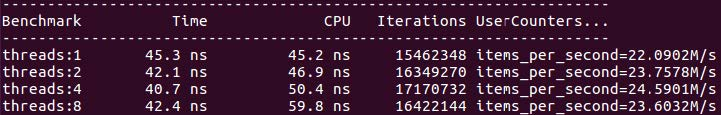
\includegraphics[width=0.9\textwidth]{content/2/chapter7/images/15.jpg}\\ 
Figure 7.15 – Performance of the lock-free stack on X86 CPU (compare with Figure 7.11)
\end{center}

For comparison, the spinlock-guarded stack can execute about 70M operations per second on the same machine. This is consistent with the expectations we had after the performance estimates in the previous section. The same estimates, however, suggested that the lock-free stack may be superior on ARM processors. The benchmark confirms that our efforts were not wasted:

\hspace*{\fill} \\ %插入空行
\begin{center}
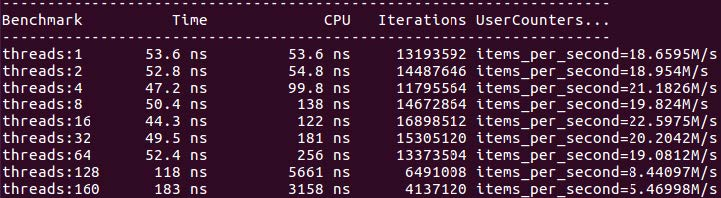
\includegraphics[width=0.9\textwidth]{content/2/chapter7/images/16.jpg}\\ 
Figure 7.16 – Performance of the lock-free stack on ARM CPU (compare with Figure 7.12)
\end{center}

While the single-threaded performance of the lock-based stack is superior, the lock-free stack is much faster if the number of threads is large. The advantage of the lock-free stack becomes even greater if the benchmark includes a large fraction of top() calls (that is, many threads read the top element before one thread pops it) or if the producer and consumer threads are distinct (some threads call only push(), while other threads call only pop()).

To conclude this section, we have explored the different implementations of a thread-safe stack data structure. To understand what is required for thread safety, we had to analyze each operation separately, as well as the interaction of multiple concurrent operations. The following are the lessons that we learned:

\begin{itemize}
\item 
With a good lock implementation, a lock-guarded stack offers reasonable performance and is much simpler than the alternatives.

\item 
Any application-specific knowledge about the limitations on the use of the data structure should be exploited to gain performance cheaply. This is not the place to develop generic solutions, quite the opposite: implement as few features as you can and try to gain performance advantages from the restrictions.

\item 
A generic lock-free implementation is possible but, even for a data structure, that is as simple as a stack, it is quite complex. Sometimes, this complexity may even be justified.

\end{itemize}

So far, we have skirted the issue of memory management: it is hidden behind the vague allocate more memory when the stack runs out of capacity. We will need to come back to that later. But first, let's explore more different data structures.


































